\section{Sequential AIR}

Let us start by describing the model from the point of view of its generative story. Images are generated by first assuming that, at every time-step, objects are propagated from previous time-step and some new objects can be introduced. Let $k \in \{0, 1, \dots, K\}$, $K \in \mathcal{N}_+$ the number of objects propagated from the previous time-step and let $n \in \{0, 1, \dots, N - k\}$, $N \in \mathcal{N}_+$ the number of objects discovered at the current time-step. The maximum of $K$ objects can be propagated and the model can handle up to $N$ total objects, therefore $K \leq N$. 

Let superscripts $D$ and $P$ denote latent variables generated by discovery and propagation models, respectively. At the first time-step $t = 1$ there are no objects to propagate, so we sample up to $N$ objects from a discovery prior $\p{n_1, \bz_1^D}{N}$. Starting from the second time-step $t=2$, the model first propagates objects by sampling from a propagation prior $\p{k_2, \bz_2^P}{n_1 + k_1, \bz_1}$, where $\bz_1 = \bz_1^D$. The model also samples $n_2$ new objects from the prior $\p{n_2, \bz_2^D}{N - k_2}$. From now on, that is for $t \geq 2$, we set the aggregated latent variable $\bz_t = \{\bz_t^P, \bz_t^D\}$. This process continues up to the final time-step $T$. The images are generated by passing the generated latent variables $\bzTs$ to the generative model $\p{\bxt}{\bzt}{\theta}$ one at a time. Note that $\bzt$ is a set of up to $N$ latent variable, where each latent variable represents a separate objects. The generating model acts separately on every latent variables in the set, and the output random variable of the generating model consists of the sum of outputs of the generative model for each latent variable in the set. \Cref{fig:seq_air} shows the graphical model of the generative story. Please note that the prior for the number of new objects stays the same for every time-step and it is analogous to the prior used by AIR, with the exception that the number of maximum objects can differ.

To make it more formal, we will now give all equations governing the generative process. The prior for the discovery model is defined as follows.
\begin{equation}
\begin{aligned}
    \p{n_t, \bzt^D}{N} &=\\
    \p{n_t}{N} \p{\bzt}{n_t} &= \mathrm{TruncatedGeom} (n_t \mid N) \prod_{i=1}^{n_t} \gauss{\bf{0}, I},
\end{aligned}
\end{equation}
where TruncatedGeom$(n_t \mid N)$ is a geometric distribution, whose support is truncated to $\{0, 1, \dots, N\}$. The propagation model is defined by the following.
\begin{equation}
\begin{aligned}
    \p{k_t, \bzt^P}{m_{t-1}, \bz_{1:t-1}} = \prod_{j=1}^m \p{\bt^j}{\bz_{1:t-1}^j} \p{\bzt^j}{\bz_{1:t-1}^j} =\\
    \prod_{j=1}^{m_{t-1}} \mathrm{Bernoulli} \left(\bt^j \mid \psi( \bz_{1:t-1}^j) \right) \gauss{\bzt^j \mid \bm{\mu} (\bz_{1:t-1}^j), \bm{\sigma}^2(\bz_{1:t-1}^j)},
\end{aligned}
\label{eq:prop_prior}
\end{equation}
with $\bz_{1:t-1}^j$ denoting the history of latent variables belonging to object $j$ and $\bz_{1:0}^j = \emptyset$. In the above we reparamterise $k_t$ as a sum of Bernoulli random variables $\bt^k$, that is $k_t = \sum_{i=1}^m \bt^j$. Since for every object the probability of propagation $\psi$ is different, $k_t$ follows a PoissonBinomial distribution with $m$ trials. Direct conditioning on the whole history of latent variables is impractical, and therefore we use a learned deterministic RNN to estimate $\psi$, $\mu$ and $\sigma^2$. the RNN shares parameters but maintains a separate hidden state for every object $j$. We can rewrite \Cref{eq:prop_prior} in terms of a simple recurrence as
\begin{equation}
\begin{aligned}
    \p{k_t, \bzt^P}{m_{t-1}, \bz_{1:t-1}} = \p{k_t, \bzt^P}{m_{t-1}, \bm{h}_t^j} =\\
    \prod_{j=1}^{m_{t-1}} \mathrm{Bernoulli} \left(\bt^j \mid \psi( \bm{h}_t^j ) \right) \gauss{\bzt^j \mid \bm{\mu} (\bm{h}_t^j), \bm{\sigma}^2(\bm{h}_t^j)},
\end{aligned}
\end{equation}
\begin{equation}
    \bm{h}_t^j = f^{\mathrm{RNN}}_\theta \left( \bz_{t-1}^j, \bm{h}_{t-1}^j \right).
\end{equation}
Any parameters in the generating model, \eg the parameters of the RNN, can be learnt jointly with the inference model (to be described shortly).
Alternatively, one could use a non-parametric prior for the discrete latent variable $\kTs$, \eg the Indian Buffet Process. 

Images are created by decoding the latent variables into small `glimpses' that are then transformed to match the size of the original image and summed up. Each latent variable $\bzt^j$ can be decomposed as $\bzt^j = \left\{ \bzt^{j, \mathrm{where}}, \bzt^{j, \mathrm{what}} \right\}$. More formally,
\begin{equation}
    \widehat{\bg}_t^j = f^{\mathrm{dec}}_\theta \left( \bzt^{j, \mathrm{what}} \right),
\end{equation}
\begin{equation}
    \byt^j = f^{\mathrm{STN}} \left( \widehat{\bg}_t^j, \bzt^{j, \mathrm{where}} \right),
\end{equation}
\begin{equation}
    \widehat{\bx}_t \sim \gauss{ \bxt \mid \sum_{j=1}^{N_t} \byt^j, \bm{\sigma}_x^2},
\end{equation}
with the decoder $f^{\mathrm{dec}}$, spatial transformer $f^{\mathrm{STN}}$ and a fixed per-pixel standard deviation $\bm{\sigma}_x^2$.

\textbf{Inference} To infer the latent variables, we have to invert the generative model. To do so, the inference model has to take into account the observations $\bxTs$ and produce sequences of sets of latent variables $\bzTs$.



\begin{figure}
    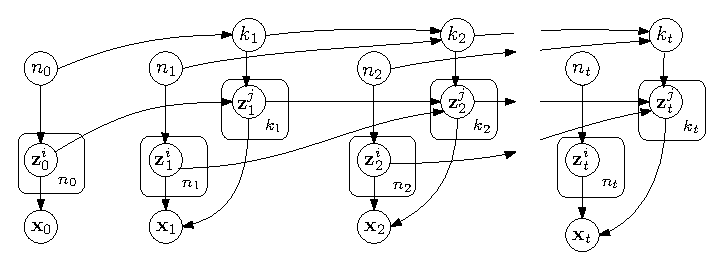
\includegraphics[width=\textwidth]{seq_air}
    \caption{The generative story of sequential AIR}
    \label{fig:seq_air}
\end{figure}

\begin{figure}
    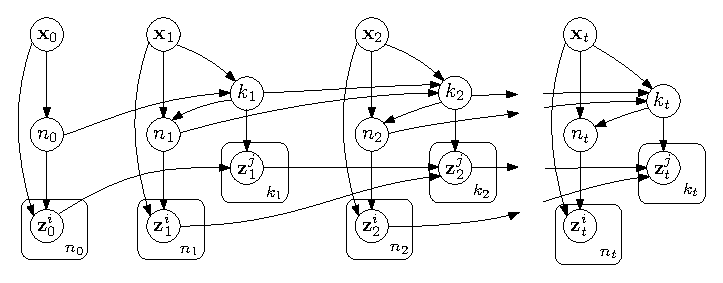
\includegraphics[width=\textwidth]{seq_air_inference}
    \caption{Graphical model for inference in sequential AIR}
    \label{fig:seq_air_inf}
\end{figure}